\tikzsetnextfilename{externalized-shortest_path}
 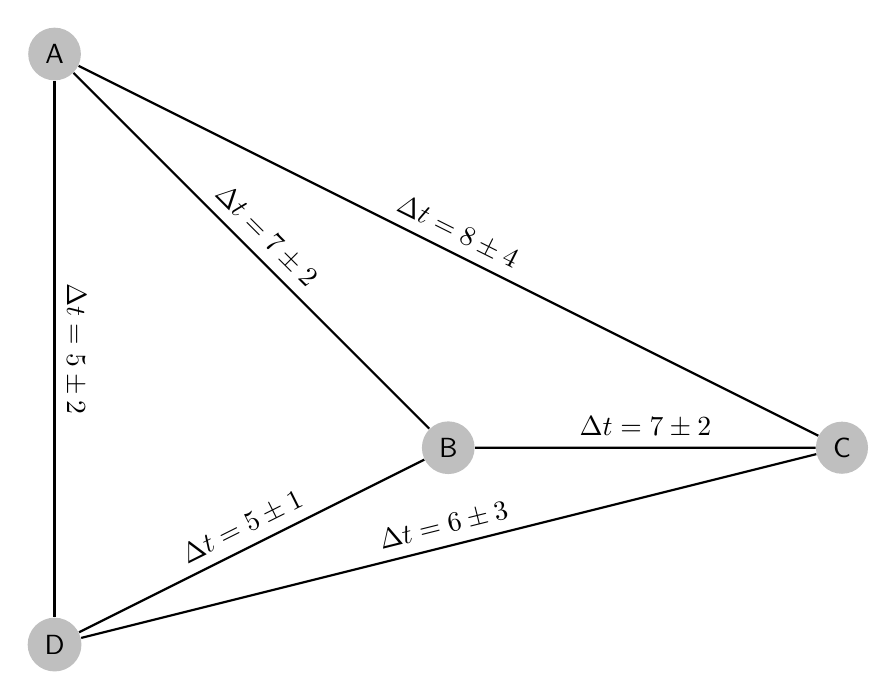
\begin{tikzpicture}
  [scale=2.5,
   font=\sffamily,
   vertex/.style={circle, fill=black!25},
   selected/.style={vertex, fill=red!24},
   edge/.style={draw, thick, -},]
  % Draw the network
  % First we draw the vertices
  \foreach \pos / \name in {{(0,3)/A}, {(2,1)/B}, {(4,1)/C}, {(0,0)/D}}
      \node[vertex] (\name) at \pos {\name};
  % Connect vertices with edges and draw weights
  \foreach \source / \dest / \offset / \error in {
        A/B/7/2,
        A/C/8/4, B/C/7/2,
        A/D/5/2, B/D/5/1, C/D/6/3}
      \path[edge] (\source) -- node[midway, above, sloped, align=left] {
        $\Delta t = \SI{\offset\pm\error}{\ns}$} (\dest);
\end{tikzpicture}
